\newcommand{\cahiersChap}{\Chapter{``Simultaneous and Systematic Abolition''?}{Cahiers de Doléances}}

\ifthenelse{\equal{\compileAsChapter}{true}}{\setcounter{chapter}{0}\cahiersChap{}}{\title{Cahiers de Doleances}\author{Jeff Jacobs\thanks{PhD Candidate, Political Science, Columbia University.}\\\texttt{jpj2122@columbia.edu}}\maketitle}

\newcommand{\cahiers}[0]{\textit{cahiers de doléances}}

\epigraph{For the ideal the French Revolution set before it was not merely a change in the French social system, but nothing short of a regeneration of the whole human race}{\cite{tocqueville_old_1856}, pp. 12--13}

\epigraph{First it changed laws, then mores, customs, and even language. Having shredded the fabric of government, it undermined the foundations of society and ultimately went after God himself. [The Revoluton was] a phenomenon so new and so different from anything that had ever happened before, yet so monstrous and incomprehensible, that the human mind could not grasp it.}{\cite{tocqueville_old_1856}, p. 13}

\epigraph{Read the \textit{cahiers}. It's all in the \textit{cahiers}.}{Jean Jules Jusserand, French Ambassador to the U.S., 1902--1924}

\section{Introduction}

Political revolt is as old as politics itself. While many have documented the histories of popular struggles, few have offered a satisfying answer to the causal question: what types of social or ideological forces could galvanize a group of people to risk life and limb directly confronting their oppressors? Speculative theories regarding the role of ideology in revolutions are not hard to come by: from Plato on Athenian revolts of 380 BC \citep{plato_republic_2007} to Hobbes on the 17th-century Leveller Revolution \citep{hobbes_leviathan_1994} to Gilbert Achcar on the Arab Spring \citep{achcar_morbid_2016}\footnote{Not to mention a rich literature on formal models of revolution, from Ted Gurr's individual-psychological account \textit{Why Men Rebel} \citep{gurr_why_1970} to Daron Acemoglu and James Robinson's institution-centered model in ``A Theory of Political Transitions'' \citep{acemoglu_theory_2001}. For a captivating exception to this material-conditions-vs.-ideology dichotomy within the literature on social movements and revolution, see Sidney Tarrow's \textit{The Language of Contention: Revolutions in Words, 1688-2012} \citep{tarrow_language_2013}.}, writers have struggled to reconcile the apparent tension between the broad socio-cultural forces that act upon all revolutionary participants and the individual agency, spontaneity, and ingenuity of each participant. Grappling with this same tension, the vast majority of empirical, or data-driven studies have focused on ``material conditions'' narrowly defined: numerically-tractable demographic, economic, and socio-cultural variables. 

In this work, we aim to take the methodological sophistication of these empirical studies and move them into the realm of rhetoric, ideology, and the history of political thought using natural language processing algorithms\footnote{On this point, however, we provide the caveat that the ``material'' and the ``ideological'' or ``cultural'' are in no way separate or even independent realms: for a simple but groundbreaking argument regarding ideology and culture itself as material phenomena, see \cite{sperber_explaining_1996}.}: what role do these less-easily-measurable factors play in galvanizing mass resistance?  %This work thus lies somewhere between the history of political thought and ``intellectual history.''
One of the biggest challenges in this area is the same as that faced by any researcher in the humanities: too many texts, not enough time\footnote{One particularly controversial ``resolution'' of this dilemma comes from the Stanford LitLab's ``distant reading'' paradigm \citep{moretti_distant_2013}, in which the researcher doesn't ``read'' texts at all in the standard sense of the word, but instead uses computational methods to derive insights from massive literary corpora. In this work we adopt the less extreme view that digital methods should serve simply as tools to aid humanists and historians in their research, in the same way that dictionaries and indices at the end of books expanded researchers' toolkits when they were introduced.}. If we aim to detect which properties of revolutionary texts are predictive of successful mass mobilization, our sample must include not only well-known influential texts (Sieyes' \textit{What is the Third Estate?} \citep{sieyes_quest-ce_1789}, the \textit{Communist Manifesto} \citep{marx_manifesto_1848}, etc.) but also the exponentially larger set of non-influential texts from the same eras, a sample too large for any one reader to digest, much less understand\footnote{Analyses which include only ``successful'' cases commit the fallacy of \textit{selection on the dependent variable}, and are fundamentally incapable of detecting which properties of the studied cases are and are not indicative of successful outcomes. Briefly: we cannot conclude that a linguistic property $X_i$ is indicative of success even in the extreme case where $X_i$ is present in every ``successful'' text, since it may simply be the case that \textit{all} texts, whether successful or not, have the property $X_i$. This fallacy is, unfortunately, extremely common and almost natural in everyday life, for example in anecdotal accounts of serial killers which claim to discern traits common to serial killers---abusive childhoods and mental illnesses, etc.---but fail to compare the prevalence of these traits in serial killers to their prevalence in society more generally.}. But developments in artificial intelligence over the past few decades---specifically in natural language processing or computational linguistics---provide social scientists an entirely new toolbox with which to dive into this ocean of text. This work will exhibit one way these tools can be used to gain insights into world-historical events, insights that would otherwise have required decades of meticulous work by dozens of researchers to obtain. 

More broadly, we intend for this research to serve as groundwork for a ``computational political theory''---a quantitatively-minded approach to political theory. This approach would view political speech acts, ideologies and political thought expressed in texts as observed manifestations of unobserved political-ideological latent variables\footnote{On the nomenclature of ``observed'' vs. ``latent'' variables, see Appendix \ref{app:pgms}, an overview of the Probabilistic Graphical Models framework from which these terms originate.}, with the latter representing various ``explanans'' of interest to political theorists: the political ideologies said to be ``held'' by the political actors under examination, for example, or their inferred positions within a broader social structure (in short, any phenomenon or set of phenomena which political theorists believe to be important for understanding the dynamics of some socio-historical situation of interest)\footnote{In the philosophy of science, the term ``explanandum'' (plural ``explananda'') denotes a phenomenon which a scientist hopes to explain, while the term ``explanans'' (plural ``explanantia'') denotes a phenomenon which is invoked by a scientist to explain an explanandum (or multiple explananda). A useful visual for understanding the relationship between observed and latent variables is the standard representation of a Hidden Markov Model, given in Figure \ref{fig:hmm} below: The variables on the top row ($X_1$, $X_2$, $X_3$) represent empirical observations—in our case political texts—while the variables on the bottom row ($S_1$, $S_2$, $S_3$) are our political-ideological latent variables, the ``underlying'' phenomena which we believe to be salient for understanding the political texts. For more on ``explanans'' vs. ``explanandia'' see \cite{elster_explaining_2015}.}.

\begin{figure}
    \centering
    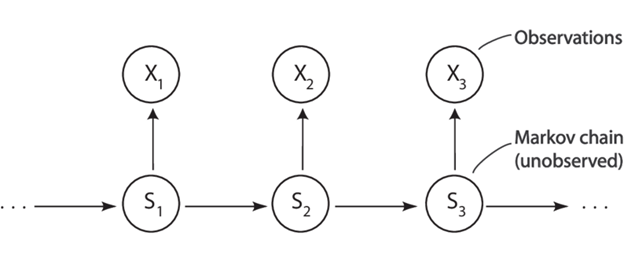
\includegraphics[width=\textwidth]{ch1_figs/markov_chain.png}
    \caption{The standard visual representation of a Hidden Markov Model. The $X_i$ variables are those we can empirically observe, like political texts, while the $S_i$ variables represent the ``underlying'' phenomena which we believe to have explanatory power with respect to the observations (the $X_i$s) (\href{https://www.researchgate.net/figure/Basic-structure-of-a-Hidden-Markov-Model_fig2_24115579}{Image source})}
    \label{fig:hmm}
\end{figure}

\section{Methods}

When conducting historical inquiry, a researcher typically begins by trying to acquire some non-insignificant portion of the extant knowledge on their subject, and subsequently spends years ``excavating'' evidence, gaining access to and examining archives. Computational methods can automate important but tedious portions of this archival work, allowing researchers to commit their full attention to the core steps of the research process: developing hypotheses, interpreting data, and drawing inductive conclusions. In other words, these algorithms can serve as ``digital research assistants,'' sifting through the massive amounts of information contained in an archive and identifying which texts and which relationships between texts are most salient to the researcher's task.

The process of empirical data analysis, whether quantitative, qualitative, or a mix of both, consists of what John Tukey calls an ``exploratory data analysis'' phase and a ``confirmatory data analysis'' phase \citep{tukey_exploratory_1977}. In the former, researchers aim to approach the data with as few preconceived notions as possible about what it ``says''. In other words, they try as hard as possible to let the data ``speak for itself'', gradually identifying patterns and associations before constructing a set of initial hypotheses. The subsequent ``confirmatory'' stage corresponds in most cases to the more standard statistical hypothesis testing procedures taught in introductory statistics courses: crafting dichotomous null and alternative hypotheses, calculating test statistics, and obtaining $p$-values.  In the following sections I discuss two separate ``classes'' of text analysis algorithms, topic models and classifiers, which can vastly expand the possibilities available to researchers in these two stages.

\subsection{Topic Modeling}

The first step to understanding any textual archive is to develop a rough schema of topics covered in the corpus, to figure out what each text is ``about'', and to group the texts accordingly. This thematic categorization, the act of transforming an archive of texts into one partitioned into sections, often takes up a massive chunk of research time and resources. Given this resource bottleneck, this transformation is precisely what one of the first text analysis methods, Latent Semantic Analysis (LSA), was created to do, and (somewhat miraculously) it does so without any input required from the researcher besides having the texts in some digitized format.

Scale-wise, LSA is already leaps and bounds beyond human capabilities, but we can do better: in 2003, David Blei, Andrew Ng, and Michael I. Jordan developed an extension to LSA called Latent Dirichlet Analysis (LDA), which ``zooms in'' on each document and actually learns distributions over topics for each token (word). That is, while LSA places each document into a single category, LDA derives a more detailed summary of each document, like ``25\% of this document is about computer science and 75\% is about linguistics,'' a more realistic model given the tendency for most written documents to range across multiple topics (for example, a news article introducing a new technology and then discussing its potential societal impact). In fact, if a researcher does want a single category for each document, they can simply choose the topic with the highest proportion: linguistics, in the case of our example document. This represents nothing short of a revolution for social science research. For a researcher hoping to study taxation practices in \textit{ancien régime} France, for example, this means the difference between reading through every text in the archive and reading through the small subset of the texts which heavily discuss a ``taxation'' topic. Depending on the time and resources available to the researcher, for example, they can read the $N$ documents with the highest proportions devoted to taxation: the more resources are available, the higher this $N$ can be.

Both LSA and LDA fall into the category of ``unsupervised'' algorithms, given the lack of user intervention in the topic-learning process. While this approach stays true to the idea of ``pure'' exploratory data analysis, it is rare for a researcher to have absolutely no idea what topics lie within an archive. More commonly, researchers come to the texts with a rough set of topics in mind and want to see which texts fall within these topics, thus shifting the nature of the research more towards confirmatory data analysis. In this case, they can use a ``semi-supervised'' Labeled LDA algorithm like CorEx \citep{gallagher_anchored_2017}, which allows them to ``suggest'' salient topics to the LDA algorithm before it runs. In our example, Labeled LDA would allow researchers to suggest single keywords like ``algorithm'' and keyword groups like \{``language'', ``linguistic''\}, thus nudging the LDA algorithm towards detecting computer science and linguistics topics.

Supervised algorithms are probably the most studied and widely-used of our three types of learning. In direct confirmatory analysis, the existence of a pre-existing codebook or categorization scheme for a corpus of interest opens up even more possibilities. Though a wide variety of supervised text analysis algorithms exist, their common goal is to learn an existing user-specified categorization scheme given only a small subset of the full corpus which has been pre-categorized, aiming to learn a categorization function which best generalizes to the larger universe of texts in the corpus. If the corpus contains one million documents, for example, the researcher could randomly sample 1000 documents from the larger corpus and manually label them using their codebook, give 800 of these documents to the algorithm as training data, then evaluate the learned classification function using the remaining 200 documents (never shown to the learning algorithm) as test data\footnote{The 800/200 split is not an arbitrary choice: this 80/20 split is recommended by most practitioners in the absence of any information about how easily the categorization scheme can be learned from a certain number of documents. This is not a mathematically-justified ``rule'', however—just a heuristic or ``rule of thumb''. Researchers with simpler categorization schemes could instead set aside 10 percent or less of the documents as training data.}.

But how exactly should we evaluate the classifier? While an intuitive measure of ``success'' is the accuracy rate of its predicted label for the 200 test documents, intuition fails in this case. A very undesirable classifier, from the researcher's perspective, could in fact still maximize this quantity. For example, if 90\% of all the documents in the corpus are about computer science, an algorithm which just guessed the label ``computer science'' for every document it ever saw would do extremely well with respect to this measure (it would be correct 90\% of the time), while failing to actually learn anything substantive about the categorization scheme. Thus, instead, computer scientists typically evaluate these learned functions using the F1 score, which incorporates both the classifier's false-positive and false-negative rates, avoiding this type of degenerate case.

\section{France 1789: The Birth of Ideology}

Shifting back to our focus at the start of the post, we now consider the question: What do texts from revolutionary eras represent? And why are they of particular interest to political theorists? From a computational political theory perspective, these texts stand out as revolutionary ``speech acts,'' representing burgeoning expressions of ideologies put out into the world intentionally as attempts to change or even destroy the extant political order. For example, when Marx closed his Communist Manifesto with the phrase ``Workers of the World, Unite!'', he was not attempting to state a true or false fact about the world, he was seeking to \textit{change} it. In the nomenclature of speech act theory, Marx's exhortation was an ``illocutionary act''. With this theory of political speech acts, utterances (e.g., sentences or phrases) whose speakers aim to \textit{do} something rather than simply describe something, we have a new tool with which to understand the role of ideology and rhetoric in the history of political thought, which we now use to try and unpack the first instance of a successful revolution built upon an ideologically-complete\footnote{Here we use ``politically complete'' in a sense similar to that of the ``completeness'' of a formal mathematical theory: a set of political axioms (for example, that legitimate power is derived from ``the people'') has this property if one can derive ``answers'' to all conceivable political problems a society may face (for example, who has the legitimate authority to declare war), at least in the eyes of its believers and practitioners. In this way, the anti-clerical egalitarian republicanism espoused by the ideologues of the Revolution qualifies, as does the ``official'' Soviet Communist doctrine which emerged under Stalin as well as the ``Islamic Liberation Theology'' of revolutionary Iran. The Cuban Revolution-based ideology of \textit{foquismo} (sometimes termed ``Guevarism''), however, is not politically-complete, since it only claims to answer the political problem of how to take power, not what to do once in power. Interestingly, Niccolo Machiavelli recognized the importance of this taking-power/using-power dichotomy and separately addressed his two major works to these topics (\textit{The Prince} as a manual for taking power, and \textit{Discourses on Livy} as a manual for governing once in power).}, universal\footnote{\cite{halliday_revolution_1999} notes that all of the ideologies cited in the prior footnote were immediately, and violently, ``exported'' to other nations/regions outside of that in which the ideology had ``officially'' taken hold. Whether this perceived and acted-upon universality is a property of \textit{all} politically-complete ideologies is an interesting question, but outside the scope of this work.} theory of a just society: the French Revolution.

So much of our contemporary understanding of politics comes from the French Revolution that we often don't even notice it. The idea of a political ``left'' and ``right'' wing, for example, comes from the tendency during the Revolution for radical republicans to sit on the left side of the National Assembly while the conservative monarchists sat on the right. This linear arrangement, however, is a rare example of order in an otherwise chaotic and violent revolution.

Beginning in a wave of vociferous intellectual energy as ordinary citizens started to challenge their most deeply-held socio-political convictions, the revolutionaries issued several constitutions over the span of a few years (in 1791, 1793, and 1795), each one more innovative and utopian than the last, each one reaching a little further toward achieving a just society. However, as the revolution approached its fifth year after the constitution of 1793, its ideological underpinnings became increasingly obscured by the shadow of violence, as fear of losing existing gains gave rise to the ``Reign of Terror.'' In scenes presaging the worst atrocities of the 20th century, citizens resolved personal grudges by denouncing friends and neighbors as traitors---specifically, as enemies of the revolution---thus ensuring a quick execution via guillotine \citep{furet_interpreting_1978}.

The journalist Jacques Mallet du Pan summed up this violent turn in his 1793 adage: ``like Saturn, the revolution devours its children''. An event of such world-historical importance has, of course, been analyzed and re-analyzed ad infinitum by historians over the years. But the incredible fact of the French Revolution from a historiographic perspective is that a sort of mass ``public opinion survey'' was taken the very year that it broke out: the \cahiers{} or ``grievance books.'' These documents, from the moment of revolutionary ignition, offer monumental benefit to historians: they give first-hand accounts of the main reported political problems and aspirations of people from all different social strata of the country, providing an incredible insight into the theoretical and practical underpinnings of the coming transformation. They also allow us to combat the hereditary narrative handed down via the conservative accounts of theorists such as Edmund Burke, who described the achievements of the revolution as ``all sorts of crimes jumbled together with all sorts of follies'', and the new revolutionary state as ``a nation of gross, stupid, ferocious, and at the same time, poor and sordid barbarians, destitute of religion, honor, or manly pride'' \citep{burke_reflections_1790}.

\section{The \textit{Cahiers}}

In light of the economic crisis knocking at his door, King Louis XVI called for the Estates General to be convened, wherein he could ask the nobles to lend him the money he needed to pay off his state debts. However, before the council could be called, ordinances stated that a record of grievances to be discussed in the meeting must be collected from the people. At the time, France had an explicit and institutionalized hierarchy of social castes called ``Estates'', with a small minority belonging to the Nobility and the Clergy and the vast majority, including the incipient bourgeoisie, belonging to a group creatively called the ``Third Estate.'' The Estates-General ordinance specifically required separate grievance books to be drafted by each of these three estates within each administrative region (called \textit{bailliages} or \textit{senechausses}) of the country, giving us not only a ``snapshot'' of France at the cusp of revolution, but a snapshot explicitly surveying specific cross-sections of society, the ideal material for researchers in the social sciences\footnote{Even today, social science researchers almost never have access to such widely representative data: survey results are typically generated via weighted averaging of the raw response data, to simulate what the data would look like if respondents were truly representative of the population.}.

\begin{figure}
    \centering
    \includegraphics[width=0.5\textwidth]{ch1_figs/corsica_te.jpg}
    \caption{(Example of an actual published ``grievance book'', this one containing the grievances of the Third Estate [\textit{Tiers-Etat}] of Corsica [L'Isle de Corse])}
    \label{fig:cahier}
\end{figure}

Thus the \cahiers{} were born, as people all over the country proclaimed their anger, often ignoring the bureaucratically-crafted template in order to voice their own concerns more fully. The practice had not been repeated until recent months, when Emmanuel Macron resurrected the call for grievances, perhaps in an attempt to placate the \textit{gilets jaunes} or ``yellow vests'' movement. Most of what we know about the \textit{cahiers} has been curated at every turn in its three centuries of life, from Alfred Cobban back to Tocqueville and even to the original nouveau bourgeoisie delegates who, in selecting which matters to present to the king, likely emphasized matters relating more to their own class than to that of the peasant class. The King, characteristically underestimating the severity of the situation, largely ignored the collected complaints, which only served to further provoke the already revolting populace to more drastic action (see Figure \ref{fig:revolts} below).

\begin{figure}
    \centering
    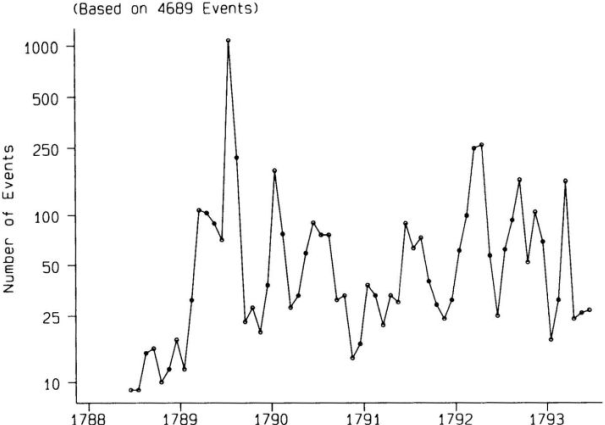
\includegraphics{ch1_figs/markoff_96_fig6-1.png}
    \caption{The frequency of peasant revolts over the course of the Revolution. The prominent spike in revolts during mid-1789 corresponds to the moment when it became clear that Louis XVI had essentially rejected all of the reforms proposed in the cahiers. (Figure from \cite{markoff_abolition_1996}, p. 271)}
    \label{fig:revolts}
\end{figure}

\subsection{Competing Interpretations of the \textit{Cahiers}}

While various theories of the causal role of the \textit{cahiers} with respect to the subsequent social upheaval have prevailed in different eras, researchers continue to uncover new texts and adopt new and usually contradictory historiographic methodologies, effectively debunking once ``confirmed'' explanations. Marxist interpretations are slowly falling away in light of postmodern suspicion of grand narratives, and today, after the so-called ``end of history'', an apathy regarding the revolution and further revolutionary activities hinders further research. Perhaps the first truly scholarly (rather than self-consciously rhetorical) attempt at providing ``the'' explanation of the Revolution came from Alexis de Tocqueville's 1856 study, \textit{The Ancien Regime and the French Revolution}. Though a member of the French intelligentsia from a noble background, and thus inevitably coming into the research with a set of preconceived notions received from his family and peers, Tocqueville aimed to conduct his study of the \textit{cahiers} in a maximally objective and methodologically-sound manner, leading some to call him ``the First Social Scientist'' \citep{elster_alexis_2009}. Nonetheless, he concluded that the documents depicted the nobility as the ``revolutionary agent'' pushing the revolution forward.

Though Tocqueville's methodological rigor far exceeded that of his contemporaries, Robert Gannett's \textit{Tocqueville Unveiled} \citep{gannett_tocqueville_2003} casts doubt on the ``representativeness'' of Tocqueville's sole source for his analysis, an abridged three-volume ``synopsis'' of the cahiers published amidst the chaos of late 1789 by political firebrand Louis-Marie Prudhomme (which, though masquerading as an informational ``résumé'', was immediately recognized as a polemical, partisan screed and promptly banned by Parisian police). Gannett concludes that ``by failing to properly assess the publisher's covert political purposes in this hastily compiled \textit{cahiers} collection, Tocqueville fell prey to the deliberate distortion injected within it'' (\cite{gannett_tocqueville_2003}, 203). This critique applies not only to Tocqueville's but to all theories which have come and gone in the decades since, given that no single person could possibly read all 40-60,000 \textit{cahiers} known to exist. Whether we want to believe Tocqueville's theory, Georges Lefebvre's Marxist theory (the dominant theory from around 1930 until 1960), George Cobban's ``Revisionist'' theory (the dominant theory from around 1960 to the present), or any other, to truly know we need some consistent methodology which will treat each of the \textit{cahiers} with equal weight.

Recognizing this issue of selection bias, quantitatively-minded historical sociologists Gilbert Shapiro and John Markoff embarked on a research endeavor which would occupy the greater part of both of their lives: the ``Revolutionary Demands'' project. With enough research assistants, they figured, and a categorical coding system which successfully struck a balance between specificity and interpretability, they could manually tag every single grievance within every single \textit{cahier} based on (a) the topic, i.e., what particular aspect of the regime the grievance was addressing, and (b) the proposed change, e.g., whether the grievance called for reformation, abolition, or expansion of an \textit{ancien régime} institution. 

Topic models, as mentioned above, are a class of algorithms which, through trying to group the semantic ideas in a text into distinct but internally cohesive topics, can identify the topics discussed across an entire corpus and measure their relative frequency of discussion. The inner workings of the algorithm rest upon a simplified story (a ``data-generating process'' or DGP) of the process of writing a sentence or paragraph: someone sits down to write about a particular topic, but they immediately forget all words except those relating to their chosen topic. So the author brainstorms, writing topic-relevant keywords, perhaps repeatedly, down as they come into their mind. Topic modeling can take the document the writer has produced and reverse engineer it such that it can determine the original constitutive ideas of the paragraph given only the groupings of words it has found.

\textit{Results and Discussion}

Topic models, then, give us a way to organize and to start to understand what would otherwise be an unmanageable mountain of texts. In the case of the cahiers de doleances, we already have an example of what humans would be able to discover given decades of painstaking labor, a blessing for those of us trying to probe the possibilities for using computers to obviate the tedious parts of research. Thus, just as Shapiro and Markoff ``transformed'' interpretations of the origins of the French Revolution from the realm of intellectual speculation to that of empirical testing and evaluation of hypotheses, we focus on two axes across which we can plot the various theories.

The first axis, social class, refers to the position of the grievance-writers within the \textit{ancien régime}. Relative to the institutional positions and national resources available to a given citizen of France, this axis is operationalized by a variable corresponding to whether the grievance is from a member of the Nobility, the Clergy, or the Third Estate\footnote{While we were able to obtain the full text of about 95\% of all Clergy cahiers---those submitted on behalf of church parishes across the country---these are vastly more numerous and less well-preserved than the \textit{cahiers} of the Nobility and the Third Estate. The \textit{cahiers} of the Clergy number in the tens of thousands, with several thousand almost certainly lost to time, while all but a few Nobility and Third Estate \textit{cahiers} are accounted for and accessible via archives throughout France. Thus, for the sake of demonstration and data quality, we restrict the analysis here to the \textit{cahiers} of the Nobility and Third Estate (our [inevitably] statistically-skewed collection of Clergy \textit{cahiers} is available upon request---for details on the existence, non-existence, and preservation status of these documents see \cite{hyslop_guide_1936}, \cite{duncan_baretta_selective_1987}, and \cite{shapiro_revolutionary_1998}, chs. 8--9).}. The second axis, however, is where the topic model really shines: social class is interacted with automatically-discovered topic, so that we can decompose a given class's grievances into, for example, grievances regarding the regime's tax structures and legal systems; those regarding the balance between royal, parliamentary, and clerical power; and those focused on more general principles of justice and human rights.

As mentioned earlier, however, these topic models are unsupervised—the statistical model chooses the topics for us, which can be a blessing or a curse depending upon the ratio of ``signal'' to ``noise'' in the corpus it is trained on. While there is still controversy over which properties of texts constitute ``signal'' and which constitute ``noise'' (see, e.g., \cite{schofield_pulling_2017} for a recent rethinking of this dichotomy, or \cite{denny_text_2018} for an empirical illustration of how different assumptions can drastically affect findings), we opted to perform a series of linguistic preprocessing steps aimed at maximizing the semantically-relevant content in each document.

First, we removed function words (``le'', ``une'', ``et'', and so on, also called ``stopwords''). In a grievance like ``Abolissez la taxe foncière!'' (``Abolish the land tax!'') the presence of ``le'' conveys no information about the topical focus of the grievance. Then, we mapped various pluralizations and conjugations of a word to a single ``stem'' word and transformed all remaining words to lowercase. Finally, we trained a phraser to detect and tag meaningful multi-word phrases like ``droit de contrôle'' or ``tiers état'' before running these steps, to ensure they would be treated as atomic linguistic units when appearing in the corpus, since, for example, ``impôt foncier'' (``land tax'') has a meaning distinct from that of either ``impôt'' or ``foncier'' appearing in isolation.

\begin{figure}
    \centering
    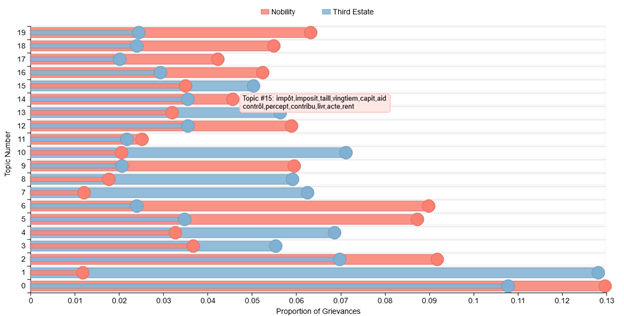
\includegraphics{ch1_figs/topic_viz.png}
    \caption{A screenshot from the interactive visualizer, available at \href{https://textlab.app/cahiers}{https://textlab.app/cahiers}}
    \label{fig:topicviz}
\end{figure}

The actual results generated by the model can be explored using our topic visualization app at \href{https://textlab.app/cahiers}{https://textlab.app/cahiers}). Though there are several striking features, perhaps the starkest result visible in the graph is the massively greater emphasis on seigneurial institutions (Topic 1)---the institutional embodiments of the feudal system itself---among Third Estate cahiers relative to the cahiers of the Nobility. While LDA topics are not mutually-exclusive, so that one must be careful not to assume a clean one-to-one mapping between the algorithmically-discovered topics and the latent topics established and discussed by scholars of the French Revolution, the gap in Topic 1 emphasis between the two estates is statistically significant, as can be seen in Figure 2 below, which provides bootstrapped confidence intervals for the 40 estimated topic proportions.

[Non-interactive version of the topic emphasis graph here]

Conversely, the topic with the highest Nobility-emphasis to Third Estate-emphasis ratio is Topic 6, which straightforwardly represents grievances discussing the Noble \textit{députés} (deputies) elected to represent the Nobility at the Estates-General and, in particular, the procedures by which voting would be conducted. While scholars continue to argue about the various rationales, the particulars of the legitimating ideologies and argumentative strategies employed to this end, proffered by the Nobility when demanding that the Estates-General retain its highly-disproportionate ``vote by estate'' rule, there is near consensus that ``vote by head'' vs. ``vote by estate'' was probably the most salient and mobilizing issue among politically-engaged French citizens during the nationwide debates from January to May 1789.

Constituting less than two percent of the Kingdom's citizens, the Nobles feared that a change to the ``vote by head'' rule would sound the death knell for their existence as a privileged class, much as White Rhodesians in 1980, White South Africans in 1994, or Jewish Israelis today have recognized the mortal threat that democratic representation would present to their continued dominance. While this result is not surprising, it does buoy our confidence in the model's veracity as a reflection of the major concerns of each estate.

A potentially more interesting result comes if we contrast the extremely high (and statistically significant) Nobility-to-Third-Estate emphasis ratio of Topic 6, which centers around voting procedures, with the extremely low (and even more statistically significant) ratio for Topic 1, focusing on seigneurial institutions. While the Nobility's energy went towards fighting for what modern theorists of democracy would call the ``procedural conception'' of democracy, where democracy is justified in broadly deontological terms as having the ability to bind people via mutually-established rules/institutions which substantively incorporate their voices, the Third Estate mobilized around an ``instrumental'' conception.  Their contrasting democratic-theoretical framework instead justified democracy e consequentially in terms of the ends that it can be put towards---in this case, the abolition or at least significant attenuation of feudal powers and privileges.

Here we have only examined two of the 20 topics learned by the topic model, yet already we have some evidence or at least some preliminary hypotheses we can bring to bear in evaluating the theories cited above, regarding the role(s) of different estates and social classes in precipitating the major events of the early Revolution. It seems reasonable to conclude that the Nobility found themselves on the defensive, trying to justify a continuation of the status quo on procedural grounds, or, perhaps more accurately, on the grounds of defending tradition,when drafting their \textit{cahiers}. The Third Estate, by contrast, devoted a tremendous proportion of their grievances towards developing a more recognizably ``modern'' rights-based argument, highlighting the onerous infringements upon their dignity and autonomy which the institutions of the feudal regime enabled and encouraged.

In consequence, claims like Tocqueville's that the Nobility was essentially ``as radical as'' the Third Estate fall flat. Instead, our findings favor the more Marxist-like arguments of Lefebvre and Cobban, positing the Revolution as essentially the result of a collision of mutually-opposed class interests. Delegates of the Nobility and the Third Estate held more-or-less irreconcilable views regarding who should steer the ship of state and how they should steer it. While this vindicates the 20th-century scholars' ``break'' from the Tocqueville-dominated ``consensus'' interpretation of the 19th century, it still leaves us with the central interpretive dispute among these 20th-century scholars, that between Lefebvre's ``orthodox'' Marxist theory and Cobban's ``revisionist'' theory focusing on the role of the peasantry. To what degree were peasants able to ``steer'' the direction of the revolution, via revolts and other forms of collective mobilization, towards outcomes which addressed their grievances, especially in comparison to the Parisian sans-culottes? How different were their aims in the first place? Until we incorporate the Parish (Clergy) \textit{cahiers} as a third data source for our analysis, we are unable to adjudicate between these two theories and unable to answer these questions. Though it's outside the scope of this post, the task of constructing a convincingly representative sample of the Parish \textit{cahiers} to enable such a study should be a central concern for quantitatively-minded historical researchers. Combining  21st-century probabilistic programming frameworks like Stan or Edward with some of the aforementioned text-as-data algorithms, one could develop a far more convincing set of joint topic-emphasis estimates for all three estates than those computed by Shapiro and Markoff, who use a somewhat opaque and ad hoc clustering method to try and correct for sampling biases\footnote{Shapiro and Markoff's procedure also, as far as we can tell, does not incorporate any explicit missing-data modeling or imputation, despite the authors' meticulous work researching and describing the ``missingness'' properties of the Parish \textit{cahiers} (in chapters 7-8 of \cite{shapiro_revolutionary_1998} and in \cite{duncan_baretta_selective_1987}). Although missing-data modeling and imputation have historically been somewhat ad hoc and heuristic-driven, Bayesian programming frameworks like Stan and Edward provide a statistically-principled missing-data model and imputation procedure ``automatically'': since all data is modeled explicitly (Bayesian models require explicit specification of probability distributions for both the data points $X = \{x_1, x_2, \ldots, x_N\}$ and the model parameters $\theta = \{\theta_1, \theta_2, \ldots, \theta_M\}$, since values for the latter are estimated using the model's posterior distribution after the Bayesian update equation has been applied, i.e., by computing $\theta^* = \max_{\theta} P(\theta | X_{obs})$, where $X_{obs}$ is the observed subset of $X$), missing data $X_m$ can be imputed by running the model ``backwards'', i.e., by subsequently computing $X_m^* = \max_{X_m} P(X_m | X_{obs}; \theta)$ once satisfactory estimates for the model parameters $\theta$ have been obtained.}.

\section{Conclusion}

The French Revolution is only one example among hundreds of people taking action in the realm of politics and fundamentally transforming the political arrangements---institutions, hierarchies, norms---with which their day-to-day lives are imbricated and co-constitutive. For the sake of actually starting to understand revolutions and political change in a meaningful way, it's imperative that we employ methodologies which ``translate'' across revolutions, instead of infinitely fine-tuning (in computer science parlance, ``overfitting'') to a particular case. 

The central point, in our view, is not so much to understand the cahiers as such but instead to develop systems allowing historical/social-scientific researchers to ``stand on the shoulders of [algorithmic] giants,'' exploring the transformations of the political-historic landscape not as hikers but as pilots, gaining a more complete view of the geography. From this vantage point, then, those who wish to make the future better than the past---organizers, advocates for social change---will be able to see with greater clarity the lay of the land, the obstacles in their way and how historical actors have navigated them with greater or lesser success. Social movements could thus be empowered to find new answers to perennial questions of organizational efficacy and decision-making, augmenting accumulated institutional memory and folk wisdom with the results of statistically-principled analyses. Otherwise, these lessons of history will remain the dominion of those select few with the time and resources necessary to perform decades-long intensive studies like those of Shapiro and Markoff.

\begin{subappendices}

\section{Probabilistic Graphical Models and Topic Models\label{app:pgms}}

\begin{figure}
    \centering
    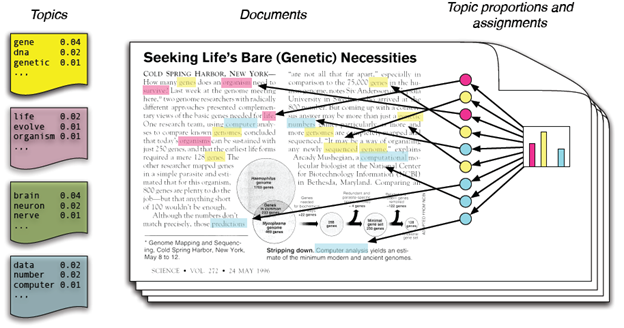
\includegraphics[width=\textwidth]{ch1_figs/blei_lda.png}
    \caption{From \cite{blei_introduction_2012}, p. 3}
    \label{fig:my_label}
\end{figure}

When trying to understand a complex phenomenon with lots of moving parts interacting with one another, a good way to start is often to break it down into its constituent elements and then specify how these elements work together to produce the phenomenon. A ``Probabilistic Graphical Model'' or PGM is a statistical tool which operationalizes this intuitive idea. A PGM is a collection of nodes (drawn as circles) representing variables and edges (drawn as arrows) representing relationships of influence between nodes, codified as ``Conditional Probability Tables''. So, if we wanted to model the relationship between weather and a person's choice of whether to go out and party or stay in and watch a movie on a given Saturday evening, we could make:

\begin{enumerate}
    \item A variable $w$ which can take on values in $\{\textsf{Sunny}, \textsf{Rainy}\}$
    \item A variable $a$ which can take on values in $\{\textsf{Go Out}, \textsf{Stay In}\}$, and 
    \item An edge $e$ from $w$ to $a$ which encodes the intuition that one is more likely to go out if it's sunny than if it's rainy via the probability distribution $P(\textsf{Go Out} \; | \; \textsf{Sunny}) = 0.75$, $P(\textsf{Stay In} \; | \; \textsf{Sunny}) = 0.25$, $P(\textsf{Go Out} \; | \; \textsf{Rainy}) = 0.25$, and $P(\textsf{Stay In} \; | \; \textsf{Rainy}) = 0.75$.
\end{enumerate}

The resulting PGM, in graphical form\footnote{The ``Graphical'' in Probabilistic Graphical Model is not used in the same sense as the ``graphical'' we're used to from vernacular English. Capital-G Graphical denotes that the Probabilistic Model is represented as a Graph, a well-defined mathematical object consisting of nodes and edges, which does not have to be represented graphically (though it could be, like in our example here with circles and arrows). In fact, when a computer program is estimating a PGM, it is by definition not in a graphical form---it's in the form of 0s and 1s, stored in the computer's memory.}, is presented in Figure \ref{fig:pgm1}, where the Conditional Probability Table describing the edge from the $w$ node to the $a$ node is given in Table \ref{tab:cpt1}.

\begin{figure}[ht!]
  \centering
  \tikz{ %
    \node[latent] (w) {$w$} ; %
    \node[latent, right=of w] (a) {$a$} ; %
    \edge {w} {a} ;
  }
  \caption{A basic PGM, representing the relationship between $w$, the weather, and $a$, the subsequent action of a person deciding whether to go out or stay in for the night.}
  \label{fig:pgm1}
\end{figure}

%\begin{figure}
%    \centering
%    \includegraphics{fig3.png}
%    \caption{A basic PGM, representing the relationship between $w$, the weather, and $a$, the subsequent action of a person deciding whether to go out or stay in for the night.}
%    \label{fig:pgm1}
%\end{figure}

\begin{table}[ht!]
    \centering
    \begin{tabular}{c|cc}
         & \textsf{Go Out} & \textsf{Stay In} \\\hline
       \textsf{Sunny} & 0.75 & 0.25 \\
       \textsf{Rainy} & 0.25 & 0.75 \\
    \end{tabular}
    \caption{The Conditional Probability Table for the PGM shown in Figure \ref{fig:pgm1}.}
    \label{tab:cpt1}
\end{table}

PGMs can help us make inferences about the world in the face of incomplete information, which is the situation in nearly every real-world problem. The key tool here is the separation of nodes into two categories: \textit{observed} (represented graphically as a shaded node) and \textit{latent} (represented graphically as an unshaded node). Thus we can now use our model as a weather-inference machine: if we observe that the person we're modeling is out at a party with us, what can we infer from this information about the weather outside? We can draw this situation as a PGM with shaded and unshaded nodes, as in Figure \ref{fig:pgm2}, and then use Bayes' Rule to perform calculations over the network, to see how the observed information about the person at the party ``flows'' back into the node representing the weather.

\begin{figure}[ht!]
  \centering
  \tikz{ %
    \node[latent] (w) {$w$} ; %
    \node[obs, right=of w] (a) {$a$} ; %
    \edge {w} {a} ;
  }
  \caption{A PGM representing the same situation as in Figure \ref{fig:pgm1}, except that the node for variable $a$ is now shaded, indicating a situation where we have observed the person's action ($a = \textsf{Go Out}$) but still only have a probability distribution over the weather $w$.}
  \label{fig:pgm2}
\end{figure}

%\begin{figure}
%    \centering
%    \includegraphics{fig4.png}
%    \caption{A PGM representing the same situation as in Figure \ref{fig:pgm1}, except that the node for variable $a$ is now shaded, indicating a situation where we have observed the person's action ($a = \textsf{Go Out}$) but still only have a probability distribution over the weather $w$.}
%    \label{fig:my_label}
%\end{figure}

Keeping in mind that Bayes' Rule tells us, for any two events $A$ and $B$, how to use information about $P(B|A)$ to obtain information about $P(A|B)$:
\begin{align*}
P(A | B) = \frac{P(B | A)P(A)}{P(B)},
\end{align*}
We can now apply this rule to obtain our new probability distribution over the weather, taking into account the new information that the person has chosen to go out:
\begin{align*}
P(w = \textsf{Sunny} \; | \; a = \textsf{Go Out}) &= \frac{P(a = \textsf{Go Out} \; | \; w = \textsf{Sunny})}{P(a = \textsf{Go Out})} \\
&= \frac{P(a = \textsf{Go Out} \; | \; w = \textsf{Sunny})}{P(a = \textsf{Go Out} \; | \; w = \textsf{Sunny}) + P(a = \textsf{Go Out} \; | \; w = \textsf{Rainy})}
\end{align*}

And now we simply plug in the information we already have from our conditional probability table to obtain our new (conditional) probability of interest:
\begin{align*}
P(w = \textsf{Sunny} \; | \; a = \textsf{Go Out}) = \frac{(0.8)(0.5)}{(0.8)(0.5) + (0.1)(0.5)} = \frac{0.4}{0.4 + 0.05} = \frac{0.4}{0.45} \approx 0.89.
\end{align*}

We have learned something interesting: now that we've observed the person out at a party, the probability that it is sunny out jumps from $0.5$ (called the ``prior'' estimate of $w$, i.e., our best guess without any other relevant information) to $0.89$ (called the ``posterior'' estimate of $w$, i.e., our best guess after incorporating relevant information).

\end{subappendices}
